\newcommand{\Release}{}
\newcommand{\Slide}{}
\newcommand{\PrintLecture}{1}
\newcommand{\PrintSolution}{1}
\newcommand{\MyCourse}{データサイエンスコース}
\newcommand{\MySemester}{春学期}
\newcommand{\MySubject}{基礎数学}
\newcommand{\MyClass}{担当教員の紹介}% フォルダ名自動挿入

\input{../../tex/hss_lualatex.tex}
\input{../../tex/hss_hyperref.tex}
\input{../../tex/hss_beamer.tex}

\AtBeginSection[]{}
\subtitle{}
\date{}

\setbeameroption{hide notes}
%\setbeameroption{show notes}
%\setbeameroption{show only notes}
%\setbeameroption{show notes on second screen=right}

\begin{document}

\maketitle

\section{担当教員}

\MyFrame{担当教員}
{
  \setstretch{1.1}

  \begin{wrapfigure}{r}{0.2\textwidth}
    \vspace{-10mm}
    \hfill
    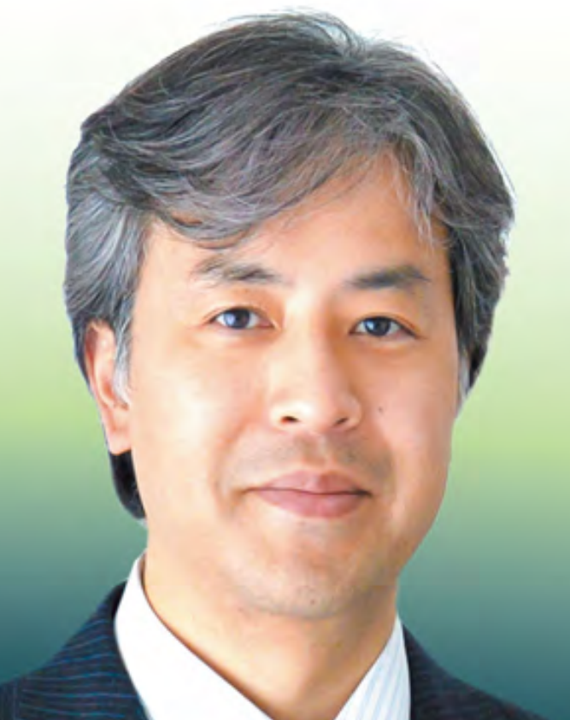
\includegraphics[width=0.2\textwidth]{self.png}
  \end{wrapfigure}

  \Large 竹田 恒(たけだ ひさし)\small\\[3mm]

  \noindent
  【研究室】第1キャンパス 管理棟A308号室\\[3mm]

  \noindent
  【Email】 htakeda@tiu.ac.jp ~
  【URL】https://stats.dip.jp\\[3mm]

  \noindent
  【学歴】\\
  ・ 筑波大学 第三学類 基礎工学類 変換工学専攻\\
  ・ 筑波大学大学院 工学研究科 構造工学専攻 修士(工学)\\
  ・ コロンビア大学大学院 統計学科 統計学修士\\
  ・ 総合研究大学院大学 複合科学研究科 統計科学専攻 博士(統計科学)\\[3mm]

  \noindent
  【経歴】\\
  ・ 東京電力HD 経営戦略調査室\\
    主幹研究員,スペシャリスト(応用統計技術)\\
  ・ 2021年10月より,東京国際大学 データサイエンス教育研究所 教授\\[3mm]

  \noindent
  【研究分野】\\
  需要予測,再生可能エネルギー予測,ソフトウェア開発
}

\section{研究分野}

\MyFrame{研究分野}
{
  電力需要,再生可能エネルギー,市場価格などの
  時系列データを用いた予測技術について研究開発,国家プロジェクトに参画\\[10mm]

  \MyFig{1.0}{電力需要データの分析(イメージ).png}
  \MyCap{電力需要データの分析(イメージ)}
}

\MyFrame{研究分野}
{
  \MyFig{0.8}{でんき予報.png}
  \MyCap{でんき予報}
  \MyRef
  {【東京電力パワーグリッド】でんき予報}
  {https://www.tepco.co.jp/forecast}
}

\section{担当授業}

\MyFrame{担当授業}
{
  \begin{itemize}
    \item 基礎数学(1年春学期)
    \item  確率・統計(1年秋学期)
    \item  ビジネス アナリティクス(2年春学期)
    \item  機械学習(2年秋学期)
    \item  R入門(3年春学期)
  \end{itemize}
}

\end{document}
